%%%%%%%%%%%%%%%%%%%%%%%%%%%%%%%%%%%%%%%%%%%%%%%%%%%%%%%%%%%%%%%
%% OXFORD THESIS TEMPLATE

% Use this template to produce a standard thesis that meets the Oxford University requirements for DPhil submission
%
% Originally by Keith A. Gillow (gillow@maths.ox.ac.uk), 1997
% Modified by Sam Evans (sam@samuelevansresearch.org), 2007
% Modified by John McManigle (john@oxfordechoes.com), 2015
% Modified by Ulrik Lyngs (ulrik.lyngs@cs.ox.ac.uk), 2018, for use with R Markdown
%
% Ulrik Lyngs, 25 Nov 2018: Following John McManigle, broad permissions are granted to use, modify, and distribute this software
% as specified in the MIT License included in this distribution's LICENSE file.
%
% John tried to comment this file extensively, so read through it to see how to use the various options.  Remember
% that in LaTeX, any line starting with a % is NOT executed.  Several places below, you have a choice of which line to use
% out of multiple options (eg draft vs final, for PDF vs for binding, etc.)  When you pick one, add a % to the beginning of
% the lines you don't want.


%%%%% CHOOSE PAGE LAYOUT
% The most common choices should be below.  You can also do other things, like replacing "a4paper" with "letterpaper", etc.

% This one will format for two-sided binding (ie left and right pages have mirror margins; blank pages inserted where needed):
%\documentclass[a4paper,twoside]{templates/ociamthesis}
% This one will format for one-sided binding (ie left margin > right margin; no extra blank pages):
%\documentclass[a4paper]{ociamthesis}
% This one will format for PDF output (ie equal margins, no extra blank pages):
%\documentclass[a4paper,nobind]{templates/ociamthesis}
%UL 2 Dec 2018: pass this in from YAML
\documentclass[a4paper, nobind]{templates/ociamthesis}
\usepackage{mathptmx}

% UL 30 Nov 2018 pandoc puts lists in 'tightlist' command when no space between bullet points in Rmd file
\providecommand{\tightlist}{%
  \setlength{\itemsep}{0pt}\setlength{\parskip}{0pt}}
 
% UL 1 Dec 2018, fix to include code in shaded environments

%UL 2 Dec 2018 reduce whitespace around verbatim environments
\usepackage{etoolbox}
\makeatletter
\preto{\@verbatim}{\topsep=0pt \partopsep=0pt }
\makeatother

%UL 26 Mar 2019, enable strikethrough
\usepackage[normalem]{ulem}

%UL 15 Oct 2019, enable link highlighting to be turned off from YAML
\definecolor{darkblue}{rgb}{0, 0, 0.5}
\usepackage[pdfpagelabels,
    colorlinks=true,
    citecolor=darkblue,
    filecolor=darkblue,
    urlcolor=darkblue,
    hidelinks=]{hyperref}
\hypersetup{
    colorlinks=true,
    citecolor=darkblue,
    filecolor=darkblue,
    urlcolor=darkblue,
    linkcolor=black,
}

%%%%% SELECT YOUR DRAFT OPTIONS
% Three options going on here; use in any combination.  But remember to turn the first two off before
% generating a PDF to send to the printer!

% This adds a "DRAFT" footer to every normal page.  (The first page of each chapter is not a "normal" page.)

% This highlights (in blue) corrections marked with (for words) \mccorrect{blah} or (for whole
% paragraphs) \begin{mccorrection} . . . \end{mccorrection}.  This can be useful for sending a PDF of
% your corrected thesis to your examiners for review.  Turn it off, and the blue disappears.
\correctionstrue

%%%%% BIBLIOGRAPHY SETUP
% Note that your bibliography will require some tweaking depending on your department, preferred format, etc.
% The options included below are just very basic "sciencey" and "humanitiesey" options to get started.
% If you've not used LaTeX before, I recommend reading a little about biblatex/biber and getting started with it.
% If you're already a LaTeX pro and are used to natbib or something, modify as necessary.
% Either way, you'll have to choose and configure an appropriate bibliography format...

% The science-type option: numerical in-text citation with references in order of appearance.
% \usepackage[style=numeric-comp, sorting=none, backend=biber, doi=false, isbn=false]{biblatex}
% \newcommand*{\bibtitle}{References}

% The humanities-type option: author-year in-text citation with an alphabetical works cited.
% \usepackage[style=authoryear, sorting=nyt, backend=biber, maxcitenames=2, useprefix, doi=false, isbn=false]{biblatex}
% \newcommand*{\bibtitle}{Works Cited}

%UL 3 Dec 2018: set this from YAML in index.Rmd
\usepackage[style=authoryear, sorting=nyt, backend=biber, maxcitenames=1, mincitenames=1, maxbibnames=100, minbibnames=100, useprefix, doi=false, url=false, isbn=false, uniquename=false]{biblatex}
\newcommand*{\bibtitle}{\textbf{Bibliography}}

% Embed reference URL under the title inside bibliography
\newbibmacro{string+url}[1]{%
  \iffieldundef{url}{#1}{\href{\thefield{url}}{#1}}
}
\DeclareFieldFormat{title}{\usebibmacro{string+url}{\mkbibemph{#1}}}
\DeclareFieldFormat*{title}{\usebibmacro{string+url}{\mkbibquote{#1}}}

% Comma between author and year in citations
\renewcommand*{\nameyeardelim}{\addcomma\space}

% This makes the bibliography left-aligned (not 'justified') and slightly smaller font.
\renewcommand*{\bibfont}{\raggedright\small}

% Change this to the name of your .bib file (usually exported from a citation manager like Zotero or EndNote).
\addbibresource{references.bib}


% Uncomment this if you want equation numbers per section (2.3.12), instead of per chapter (2.18):
%\numberwithin{equation}{subsection}


%%%%% THESIS / TITLE PAGE INFORMATION
% Everybody needs to complete the following:
\title{Application of GLM Advancements\\
to Non-Life Insurance Pricing}
\author{Leonardo Stincone}
\universityname{Università degli Studi di Trieste}
\departmentname{Scienze Economiche, Aziendali, Matematiche e Statistiche}
\degreedef{Tesi di Laurea}
\degreename{Scienze Statistiche e Attuariali}
\degreeclass{LM-83}
\academicyear{2019 - 2020}
\degreedate{March 2021}
\advisorname{Prof.~Francesco Pauli}
%\coadvisorname{}
\degreedate{March 2021}

%%%%% YOUR OWN PERSONAL MACROS
% This is a good place to dump your own LaTeX macros as they come up.

% To make text superscripts shortcuts
	\renewcommand{\th}{\textsuperscript{th}} % ex: I won 4\th place
	\newcommand{\nd}{\textsuperscript{nd}}
	\renewcommand{\st}{\textsuperscript{st}}
	\newcommand{\rd}{\textsuperscript{rd}}


% For the Title Page with Italian style (frontespizio)
\usepackage[nouppercase]{frontespizio}


%%%%%%%%%%%%%%%%%%%%%%%%%%%%%%%%%%%%%%%%%%%
%%%%% THE ACTUAL DOCUMENT STARTS HERE %%%%%
%%%%%%%%%%%%%%%%%%%%%%%%%%%%%%%%%%%%%%%%%%%
\usepackage{amsthm}
\newtheorem{theorem}{Theorem}[chapter]
\newtheorem{lemma}{Lemma}[chapter]
\newtheorem{corollary}{Corollary}[chapter]
\newtheorem{proposition}{Proposition}[chapter]
\newtheorem{conjecture}{Conjecture}[chapter]
\theoremstyle{definition}
\newtheorem{definition}{Definition}[chapter]
\theoremstyle{definition}
\newtheorem{example}{Example}[chapter]
\theoremstyle{definition}
\newtheorem{exercise}{Exercise}[chapter]
\theoremstyle{remark}
\newtheorem*{remark}{Remark}
\newtheorem*{solution}{Solution}
\begin{document}

%%%%% CHOOSE YOUR LINE SPACING HERE
% This is the official option.  Use it for your submission copy and library copy:
\setlength{\textbaselineskip}{18pt plus2pt}
% This is closer spacing (about 1.5-spaced) that you might prefer for your personal copies:
%\setlength{\textbaselineskip}{18pt plus2pt minus1pt}

% You can set the spacing here for the roman-numbered pages (acknowledgements, table of contents, etc.)
\setlength{\frontmatterbaselineskip}{16pt plus1pt minus1pt}

% UL: You can set the line and paragraph spacing here for the separate abstract page to be handed in to Examination schools
\setlength{\abstractseparatelineskip}{13pt plus1pt minus1pt}
\setlength{\abstractseparateparskip}{0pt plus 1pt}

% UL: You can set the general paragraph spacing here - I've set it to 2pt (was 0) so
% it's less claustrophobic
\setlength{\parskip}{2pt plus 1pt}


% Leave this line alone; it gets things started for the real document.
\setlength{\baselineskip}{\textbaselineskip}


%%%%% CHOOSE YOUR SECTION NUMBERING DEPTH HERE
% You have two choices.  First, how far down are sections numbered?  (Below that, they're named but
% don't get numbers.)  Second, what level of section appears in the table of contents?  These don't have
% to match: you can have numbered sections that don't show up in the ToC, or unnumbered sections that
% do.  Throughout, 0 = chapter; 1 = section; 2 = subsection; 3 = subsubsection, 4 = paragraph...

% The level that gets a number:
\setcounter{secnumdepth}{3}
% The level that shows up in the ToC:
\setcounter{tocdepth}{3}


%%%%% ABSTRACT SEPARATE
% This is used to create the separate, one-page abstract that you are required to hand into the Exam
% Schools.  You can comment it out to generate a PDF for printing or whatnot.

% JEM: Pages are roman numbered from here, though page numbers are invisible until ToC.  This is in
% keeping with most typesetting conventions.
\begin{romanpages}

% % Title page is created here
% \maketitle


% Title Page with Italian style (frontespizio
\begin{frontespizio}
  \begin{Preambolo*}
    \renewcommand {\frontinstitutionfont } {\fontsize {20}{21}\bfseries }
    \renewcommand {\frontdivisionfont } {\fontsize {16}{23}\normalfont }
    \renewcommand {\frontpretitlefont } {\fontsize {16}{23}\scshape }
    \renewcommand {\fronttitlefont } {\fontsize {24}{27}\bfseries }
    \renewcommand {\frontfixednamesfont} {\fontsize {16}{23}\normalfont }
    \renewcommand {\frontnamesfont} {\fontsize {16}{23}\bfseries }
    \renewcommand {\frontfootfont} {\fontsize {14}{20}\bfseries }
  \end{Preambolo*}
  
  \Universita{Trieste}
  %\Logo{logounits200dpi.png}
  %\Logo[4cm]{logo-units_0.png}
  \Logo[4cm]{figures/university-logo.png}
  \Dipartimento{Scienze Economiche, Aziendali, Matematiche e Statistiche}
  \Corso[Laurea Magistrale]{Scienze Statistiche e Attuariali}
  \Titoletto{Tesi di Laurea}
  \Titolo{Application of GLM Advancements\\
to Non-Life Insurance Pricing}
  \NCandidato{Candidato}
  \Candidato{Leonardo Stincone}
  \Relatore{Prof.~Francesco Pauli}
  \Annoaccademico{2019 - 2020}
\end{frontespizio}




%% Comment if you don't need a white page between title page and next pages
\null\newpage


%%%%%% Quote in the page after the title page
  \begin{quote}
    \begin{flushright}
      \textit{The data scientist is a person who is better at statistics than any software engineer\\
and better at software engineering than any statistician.}
    
      Josh Wills
    \end{flushright}
  \end{quote}


% Default spacing for non-quote chapters and sections:
% 0 space before, 40pt space after title
% set at beginning of individual chapters where needed
\titlespacing*{\chapter}{0pt}{0pt}{35pt}

%%%%% DEDICATION -- If you'd like one, un-comment the following.

%% Comment if you don't need a white page
\null\newpage

%% Comment if you don't need a white page
\null\newpage


%%%%% ACKNOWLEDGEMENTS -- Nothing to do here except comment out if you don't want it.
\begin{acknowledgements}
 	Qua potrei ringraziare:

  \begin{itemize}
  \item
    Genertel per avermi dato i dati e supportato in questa ricerca
  \item
    DEAMS per la formazione e l'apertura alla collaborazione col mondo aziendale
  \end{itemize}
\end{acknowledgements}

% %% Comment if you don't need a white page
% \null\newpage

%%%%% ABSTRACT -- Nothing to do here except comment out if you don't want it.
\begin{abstract}
  This is my abstract \dots
\end{abstract}

% %% Comment if you don't need a white page
% \null\newpage


%%%%% MINI TABLES
% This lays the groundwork for per-chapter, mini tables of contents.  Comment the following line
% (and remove \minitoc from the chapter files) if you don't want this.  Un-comment either of the
% next two lines if you want a per-chapter list of figures or tables.

% This aligns the bottom of the text of each page.  It generally makes things look better.
\flushbottom

% This is where the whole-document ToC appears:
\renewcommand{\contentsname}{\textbf{Table of Contents}}
\renewcommand{\listfigurename}{\textbf{List of Figures}}
\renewcommand{\listtablename}{\textbf{List of Tables}}
\tableofcontents

\listoffigures
	\mtcaddchapter
  	% \mtcaddchapter is needed when adding a non-chapter (but chapter-like) entity to avoid confusing minitoc

% Uncomment to generate a list of tables:
\listoftables
  \mtcaddchapter
%%%%% LIST OF ABBREVIATIONS
% This example includes a list of abbreviations.  Look at text/abbreviations.tex to see how that file is
% formatted.  The template can handle any kind of list though, so this might be a good place for a
% glossary, etc.
% Leonardo Stincone, 18/04/2021
% This code must be included in the preamble
% Package needed for abbreviations
\usepackage{acro}

% Defining the abbreviations
\DeclareAcronym{glm}{
  short = GLM,
  long = Generalized Linear Model,
}

\DeclareAcronym{aic}{
  short = AIC,
  long = Akaike Information Criterion,
}

\DeclareAcronym{bic}{
  short = BIC,
  long = Bayesian Information Criterion,
}

\DeclareAcronym{gam}{
  short = GAM,
  long = Generalized Additive Model,
}

\DeclareAcronym{map}{
  short = MAP,
  long = Maximum a Posteriori,
}

\DeclareAcronym{gbm}{
  short = GBM,
  long = Gradient Boosting Machine,
}

\DeclareAcronym{lasso}{
  short = LASSO,
  long = Least Absolute Shrinkage and Selection Operator,
}

\DeclareAcronym{rf}{
  short = RF,
  long = Random Forest,
}

\DeclareAcronym{nn}{
  short = NN,
  long = Neural Network,
}

\DeclareAcronym{mtpl}{
  short = MTPL,
  long = Motor Third Party Liability,
}

\DeclareAcronym{mod}{
  short = MOD,
  long = Motor Own Damage,
}

\DeclareAcronym{ibnyr}{
  short = IBNyR,
  long = Incurred But Not yet Reported claim,
}

\DeclareAcronym{ibner}{
  short = IBNeR,
  long = Incurred But Not enough Reported claim,
}

\DeclareAcronym{adas}{
  short = ADAS,
  long = Advanced Driver-Assistance Systems,
}

\DeclareAcronym{it}{
  short = IT,
  long = Information Technology,
}

\DeclareAcronym{etl}{
  short = ETL,
  long = Extract Transform Load,
}

\DeclareAcronym{ram}{
  short = RAM,
  long = Random Access Memory,
}

\DeclareAcronym{hdd}{
  short = HDD,
  long = Hard Disk Drive,
}

\DeclareAcronym{ssd}{
  short = SSD,
  long = Solid State Drive,
}

\DeclareAcronym{cpu}{
  short = CPU,
  long = Central Processing Unit,
}

\DeclareAcronym{haas}{
  short = HaaS,
  long = Hardware as a Service,
}


% The Roman pages, like the Roman Empire, must come to its inevitable close.
\end{romanpages}

% Setting linkcolor here so that Fig & Chap refs are colored when hidelinks=false
% but toc entries are always black
\hypersetup{
    linkcolor=darkblue,
}

%%%%% CHAPTERS
% Add or remove any chapters you'd like here, by file name (excluding '.tex'):
\flushbottom

% all your chapters and appendices will appear here
\hypertarget{introduction}{%
\chapter*{Introduction}\label{introduction}}
\addcontentsline{toc}{chapter}{Introduction}

\adjustmtc

La mia introduzione \ldots{}

\hypertarget{thesis-aim}{%
\section*{Thesis aim}\label{thesis-aim}}
\addcontentsline{toc}{section}{Thesis aim}

Lorem ipsum \ldots{}

\hypertarget{actuary-and-datascientist-figure}{%
\section*{Actuary and datascientist figure}\label{actuary-and-datascientist-figure}}
\addcontentsline{toc}{section}{Actuary and datascientist figure}

Lorem ipsum \ldots{}

\hypertarget{thesis-structure}{%
\section*{Thesis structure}\label{thesis-structure}}
\addcontentsline{toc}{section}{Thesis structure}

Lorem ipsum \ldots{}

--\textgreater{}

\hypertarget{chap:nlip-ita-market}{%
\chapter{\texorpdfstring{\textbf{Non-Life Insurance Pricing}}{Non-Life Insurance Pricing}}\label{chap:nlip-ita-market}}

\minitoc  

\chaptermark{Non-Life Insurance Pricing}

In this chapter I am going to provide an overview on how non-life insurance works from an actuarial point of view with a specific focus on the pricing process.

\hypertarget{chap:non-life-ins}{%
\section{What a Non-Life Insurance is}\label{chap:non-life-ins}}

The Italian Civil Code provides the following definition of insurance contract:

\begin{definition}[Insurance Contract, Art. 1882, Italian Civil Code]
\label{def:ins-contr} \iffalse (Insurance Contract, Art. 1882, Italian Civil Code) \fi{} The insurance is the contract with which an insurer, in exchange of the payment of a certain premium, obliged himself, within the agreed limits:
\setlist{nolistsep}

\begin{enumerate}[noitemsep]
  \item to pay an indemnity to the insured equivalent to the damage caused by an accident;
  \item or to pay an income or a capital if a life-related event occurs.
\end{enumerate}
\end{definition}

This definition identifies two parties: the \emph{Insurer} and the \emph{Policyholder}. The policyholder pays to the Insurer a certain \emph{Premium} at the beginning of the insurance coverage and the insurer will pay a benefit if a certain event (\emph{Claim}) occurs. This event could happen zero, one or more than one times, so it is possible to have more than one claim.

Usually, in non-life insurance, the benefit is the payment of a sum. This sum could be predetermined (e.g.~in motor theft insurance, where the benefit is usually the value of the insured vehicle) or defined by the entity of the claim (e.g.~in motor third party liability insurance, it depends on the damage the policyholder has provided to a third party). Regarding the ``agreed limits'', another peculiarity of non-life insurances is that the coverage period is defined as a fixed amount of time, usually corresponding to 1 year.

Starting from this legal definition, we can formalize a non-life insurance contract as follows.

Let's:

\begin{itemize}
\tightlist
\item
  \(\left]t_1, t_2\right]\), with \(t_1<t_2\), be the coverage period;
\item
  \(P>0\) be the premium payed by the policyholder to the insurer;
\item
  \(N\in\mathbb{N}\) be the number of claims occurred during the coverage period (\emph{claims count});
\item
  \(\tau_1, \tau_2, \dots, \tau_N\), with \(t_1<\tau_1< \tau_2 < \dots < \tau_N<t_2\), be the timing of each claim;
\item
  \(Z_1, Z_2, \dots, Z_N > 0\) be the amount of each claim (\emph{claims severities} or \emph{claims sizes}).
\end{itemize}

The total cost of claims for the insurance is:
\[
S = 
\begin{cases}
  0                    & \text{if } N=0 \\
  \sum_{i=1}^{N}{Z_i}  & \text{if } N>0
\end{cases}
\]
For semplicity, in the following we are going to just use the notation \(S = \sum_{i=1}^{N}{Z_i}\) with the meaning of \(0\) if \(N=0\).

Figure \ref{fig:ins-cashflow} shows the cash flows corresponding to the insurance contract. From this representation we can interpret the entering into an insurance contract by the policyholder as a way to exchange the negative cash flows \(-Z_1, -Z_2, \dots, -Z_N\) with one single negative cash flow \(-P\). On the other hand, the insurer undertakes the negative cash flows \(-Z_1, -Z_2, \dots, -Z_N\) in exchange for a positive cash flow \(+P\).

The major difference between these cash flows is that \(P\) is a certain amount, while \(Z_1, Z_2, \dots, Z_N\), at the time \(t_1\), are uncertain in the amount, in the count (\(N\)) and in the timing (\(\tau_1, \tau_2, \dots, \tau_N\)). So, the policyholder, paying a premium \(P\), is giving his risk to the insurer.

This representation points out the inversion of the production cycle typical of the insurance activity. From the insurer point of view, the revenue emerges at the beginning of the economic activity, in \(t_1\), while the costs will emerge later. In most of other economic activities, the costs emerge before the selling of the product, so the agent can choose the selling price taking into account how much that product costed him. In insurance activity, the insurer, when is selling his product (the insurance coverage), doesn't know the amount of costs he is going to pay for that product. Thus, it is crucial to properly estimate the future costs and determine an adequate premium.

From a statistical point of view, we can translate this uncertainty saying that \(N\) and \(Z_1, Z_2, \dots, Z_N\) are random variables. Therefore, we can say that \(\left\{N, Z_1, Z_2, \dots \right\}\) is a stochastic process. Usually, in non-file insurance pricing, the variables \(\tau_1, \tau_2, \dots, \tau_N\) are not taken into account because the coverage span is short and from a financial point of view the timing of the claims occurrences is negligible.

Previously we said that \(Z_1, Z_2, \dots, Z_N\) are all \(>0\). This assumption corresponds to the fact that we are excluding the null claims, i.e.~the claims that have been opened, but result in no payment due by the insurer. For the values of \(Z_i\) with \(N<i\) we can use the rule that \(\{N<i\} \Rightarrow \{Z_i = 0\}\), so \(Z_{N+1}=0, \, Z_{N+2}=0, \, \dots\). Therefore, we can say that:
\[
\{N<i \} \Longleftrightarrow \{Z_i = 0\}
\]

\begin{figure}
\centering
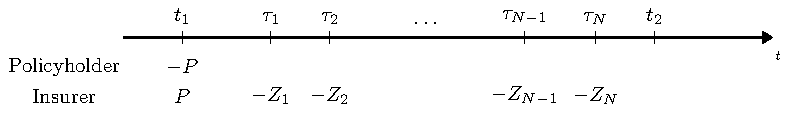
\includegraphics{_main_files/figure-latex/ins-cashflow-1.pdf}
\caption{\label{fig:ins-cashflow}Insurance Contract cash flows.}
\end{figure}

\hypertarget{non-life-insurance-pricing}{%
\section{Non-Life insurance pricing}\label{non-life-insurance-pricing}}

In insurances, the premium that the the insurer offers to the policyholder in exchange for the insurance coverage is not the same for every policyholder. The insurer evaluates the risk related to that policy and determine a ``proper'' premium taking into account risk related factors and commercial related factors. The process of \emph{pricing} corresponds in defining the set of rules for determining this ``proper'' premium \(P_i\) for a specific policyholder \(i\), given the known information on him. In the next sections I am going to better explain what ``proper'' means.

\hypertarget{compound-distribution-hypotheses}{%
\subsection{Compound distribution hypotheses}\label{compound-distribution-hypotheses}}

The first step for evaluating the stochastic process \(\left\{N, Z_1, Z_2, \dots \right\}\) is to introduce some probabilistic hypotheses. The usual hypotheses assumed are the following:

\begin{definition}[Compound distribution]
\label{def:comp-dist} \iffalse (Compound distribution) \fi{}
Let's assume that:

\begin{enumerate}
\def\labelenumi{\arabic{enumi}.}
\tightlist
\item
  for each \(n>0\), the variables \(Z_1|N=n,\ Z_2|N=n,\ \dots,\ Z_n|N=n\) are stochastically independent and identically distributed;
\item
  the probability distribution of \(Z_i|N=n, \ i\le n\) does not depend on \(n\).
\end{enumerate}

Under these hypotheses we say that:
\[
S = \sum_{i=1}^{N}{Z_i}
\]
has a compound distribution.
\end{definition}

The variable \(Z_i|N=n\) used in this definition can be interpreted as the \emph{claim severity for the \(i\)\textsuperscript{th} claim under the hypothesis that \(n\) claims occurred}. The two hypotheses provided in definition \ref{def:comp-dist} imply that the distribution of \(Z_i|N=n, \ i<n\) does not depend from \(i\) nor from \(n\). For this reason, in the following, we are going to use the notation \(Z\) to represent a random variable with the \(Z_i|N=n, \ i<n\) distribution and \(F_Z(\cdot)\) for its cumulative distribution function (i.e.~\(F_Z(z) = P(Z\le z)\)).

Let's consider the variabile \(Z_i|N>i\). We can interpret it as the \emph{claim severity for the \(i\)\textsuperscript{th} claim under the hypothesis that the \(i\)\textsuperscript{th} claim occurred}. From the hypotheses provided in definition \ref{def:comp-dist} we can obtain that also \(Z_i|N>i\) has the same distribution of \(Z_i|N=n, \ i<n\). This can be easily obtained as follows:

\begin{eqnarray}
\label{eq:z1}
P\left(Z_i \middle| N\ge i \right) & = & P\left(Z_i \middle| \bigvee_{n = i}^{+\infty}{(N=n)}\right)
\ = \\ \label{eq:z2} & = &
\sum_{n=i}^{+\infty}{ \underbrace{P\left(Z_i\le z \middle| N=n\right)}_{=F_Z(z)} P\left( N = n \middle| N\ge i \right)}
\ = \\ \label{eq:z3} & = &
\sum_{n=i}^{+\infty}{ F_Z(z) P\left( N = n \middle| N\ge i \right)}
\ = \\ \label{eq:z4} & = &
F_Z(z) \underbrace{\sum_{n=i}^{+\infty}{P\left( N = n \middle| N\ge i \right)}}_{=1}
\ = \\ \nonumber & = &
F_Z(z)
\end{eqnarray}

Where:

\begin{itemize}
\tightlist
\item
  the step \eqref{eq:z1} and the step \eqref{eq:z2} are given by the fact that the event \(\{N\ge i\}\) can be decomposed as \(\{N\ge i\} = \left\{ \bigvee_{n = i}^{+\infty}{(N=n)} \right\}\) and that the events \(\{N=n\}, n\in\{i, i+1, i+2, \dots\}\) are two-by-two disjoint, so they constitute a partition of \(\{N\ge i\}\), that allows us to use the disintegrability property of the probability;
\item
  the step \eqref{eq:z3} is due to the fact that the distribution of \(Z_i\le z | N=n\) depends neither on \(i\) nor on \(n\);
\item
  the equivalence \(\sum_{n=i}^{+\infty}{P\left( N = n \middle| N\ge i \right)} = 1\) at step \eqref{eq:z4} is due to the fact that the events \(\{N=n\}, n\in\{i, i+1, i+2, \dots\}\) are a partition of \(\{N\ge i\}\).
\end{itemize}

Therefore, \(Z\) can be considered as the \emph{claim severity for a claim under the hypothesis that that claim occurred}.

\hypertarget{chap:tcc-dist}{%
\subsection{Distribution of the total cost of claims}\label{chap:tcc-dist}}

Under the hypotheses defined in definition \ref{def:comp-dist}, it is possible to obtain the full distribution of \(S\) given the distribution of \(N\) and \(Z\). In this chapter we are going to provide only the formula of the expected value \(E(S)\), but, with the same approach one can obtain all the moments.

The expected value of the total cost of claims \(E(S)\) can be obtained from the expected value of the claims count \(E(N)\) and the expected value of the claim severity \(E(Z)\) as follows:

\begin{eqnarray}
\label{eq:s1}
E(S) & = & \sum_{n=0}^{+\infty}{P(N=n) \, E\left(S \middle| N = n \right)}
\ = \\ \label{eq:s2} & = &
\sum_{n=0}^{+\infty}{P(N=n) \, E\left(\sum_{i=1}^{n}{Z_i} \middle| N = n \right)}
\ = \\ \label{eq:s3} & = &
\sum_{n=0}^{+\infty}{P(N=n) \sum_{i=1}^{n}{\underbrace{E\left( Z_i \middle| N = n \right)}_{=E(Z)}}}
\ = \\ \label{eq:s4} & = &
\sum_{n=0}^{+\infty}{P(N=n) n E(Z)}
\ = \\ \label{eq:s5} & = &
E(Z) \underbrace{\sum_{n=0}^{+\infty}{n P(N=n)}}_{=E(N)}
\ = \\ \label{eq:s6} & = &
E(N)E(Z)
\end{eqnarray}

Where:

\begin{itemize}
\tightlist
\item
  the step \eqref{eq:s1} is given by the fact that the events \(\{N=0\}, \{N=1\}, \{N=2\}, \dots\) constitute a partition of the certain event \(\Omega\), that allows us to use the disintegrability property of the expected value;
\item
  the step \eqref{eq:s2} is due to the definition of \(S\);
\item
  the step \eqref{eq:s3} is due to the linearity of the expected value;
\item
  the steps \eqref{eq:s4} and \eqref{eq:s5} are due to the fact that, as assumed by the compound distribution hypotheses, \(E\left( Z_i \middle| N = n \right)\) does not depends on \(i\) and \(n\);
\item
  the step \eqref{eq:s6} is due to the definition of the expected value \(E(N)=\sum_{n=0}^{+\infty}{n P(N=n)}\).
\end{itemize}

This result tells us that, under the hypotheses of the compound distribution, it is possible to easily obtain \(E(S)\) from \(E(N)\) and \(E(Z)\). That means that we can model separately \(E(N)\) and \(E(Z)\) and, from them, obtain \(E(S)\). That result is particularly useful in personalization (paragraph \ref{chap:personalization}), because, for each individual \(i\), given the information we have on him \(x_i=(x_{i1}, x_{i2}, \dots, x_{ip})\), we can estimate his expected claim size \(E(N_i)\) and his expected claim severity \(E(Z_i)\) and obtain his expected total cost of claims as \(E(S_i) = E(N_i) E(Z_i)\).

\hypertarget{risk-premium-and-technical-price}{%
\subsection{Risk premium and Technical Price}\label{risk-premium-and-technical-price}}

The expected cost of claims \(E(S)\) is important because it gives us a first interpretation of what ``proper'' premium means.

\begin{definition}[Risk Premium]
\label{def:risk-premium} \iffalse (Risk Premium) \fi{} Said \(S\) the total cost of claims of a policyholder, his \emph{Risk Premium} is given by:
\[
P^{(risk)} = E(S)
\]
\end{definition}

The \emph{Risk Premium} is the premium that on average covers the total cost of claims. As mentioned above, as the coverage spans are usually short, we are not taking into account the timing of the claims and we don't discount the fact that the claims occur later than the premium payment.

It is clear that this premium, that only covers the cost of claims, is not ``proper'' in the practice.

First of all, the insurer has to cover also the expenses related to the policy (commission on sales and expenses related to the claim settlement) and the general expenses of the company. Adding the expenses, we obtain the \emph{Technical Price}.

\begin{definition}[Technical Price]
\label{def:technical-price} \iffalse (Technical Price) \fi{} Said \(S\) the total cost of claims of a policyholder and \(E\) the expenses related to his policy, his \emph{Technical Price} is given by:
\[
P^{(tech)} \ = \ E(S) + E \ = \ P^{(risk)} + E
\]
\end{definition}

Secondly, even if the policyholder would pay a premium that on average covers claims and expenses, undertaking that risk with nothing in return would not make sense for the insurer. So, to the Technical Price, a loading must be added. This loading can be justified as a loading for the risk or as a profit loading.

The result of the Technical Price with these loadings can be further modified based on business logic, as I am going to discuss later.

\hypertarget{chap:personalization}{%
\section{Modeling and Personalization}\label{chap:personalization}}

In this section We are going to better explain how pricing based on policyholder information works.

\hypertarget{pricing-variables}{%
\subsection{Pricing variables}\label{pricing-variables}}

Usually for every policyholder we have a certain amount of information on him that is considered relevant for his risk evaluation. This information must be reliable and observable at the moment of the underwriting of the policy.

In motor insurances, this information could be:

\begin{itemize}
\tightlist
\item
  Information on the insured vehicle: make, model, engine power, vehicle mass, age of the vehicle;
\item
  General information of the policyholder: age, sex, address (region, city, postcode), ownership of a private box where he parks the car;
\item
  Insurance specific information of the policyholder: number of claims caused in the previous years, how long he has been covered, bonus-malus class;
\item
  Policy options: amount of the maximum coverage, presence and amount of a deductible, presence of other insurance guarantees, how many drivers will drive the vehicle;
\item
  Customer information on the policyholder: how many years he has been a customer of the insurer, how many other policies he owns.
\item
  Telematic data: how many kilometers per year the policyholder travelled in the previous years, how many sharp accelerations and decelerations per kilometer the policyholder performed in the previous years.
\end{itemize}

These pieces of information are usually called \emph{pricing variables}.

We must observe that some of these variables are available for every potential customer (such as his age and address), while others are only available for policyholder that are already customers (such as telematic data that is available only if the policyholder agreed on installing on their car the device that collects this data).

Moreover, even considering the variables that are available for every customer, it is important to be aware on how reliable they are. Some of them comes from official documents (as customer age and address or bonus-malus class), but others could be declared by the customer and his statements are not easily verifiable by the insurer (as the ownership of a private box or how many drivers will drive the vehicle).

This topic of variables reliability fits in the wider framework of fraud detection. Insurance companies put a lot of effort in preventing frauds. This is done with active actions, such as documents checks and inspections, and with predictive fraud detections models. The two most common categories of frauds are underwriting frauds (such as false declaration on insurance related data) and settlement frauds (such as faking an accident). The customer information on the policyholder is usually important to predict both underwriting frauds and settlement frauds. Usually customers that have a longer relationship with the company and own many policies are less likely to commit frauds.

Regarding the topic of variables reliability, the Italian Insurance Associations (\href{https://www.ania.it/}{ANIA}) in the last years made some big steps forward by collecting in its databases a lot of information about policyholders and vehicles and making it available to insurance companies. For example, by logging in these databases it is possible, at the moment of the quote request, to retrieve useful insurance specific information such as the number of claims caused by the customer in the previous years or how long he has been covered and useful information on his vehicle such as when it has been registered or how many changes of ownership did it experienced.

One of the roles of the actuary is to understand how reliable the information on the policyholder is and to decide how to use that information.

\hypertarget{pricing-variables-encoding}{%
\subsection{Pricing variables encoding}\label{pricing-variables-encoding}}

Formally the pricing variables can be encoded as a vector of real numbers. \(\boldsymbol{x}_i=(x_{i1}, x_{i2}, \dots, x_{ip})\in\mathcal{X}\subseteq\mathbb{R}^p\). In the modeling framework they can be also called explanatory variables, covariates, predictors or features.

The pricing variables can be of two types:

\begin{enumerate}
\def\labelenumi{\arabic{enumi}.}
\tightlist
\item
  \emph{Quantitative variables}: variables, like policyholder age or vehicle mass, that can be easily represented as a number;
\item
  \emph{Qualitative variables}: variables, like policyholder sex or vehicle make, that represent a category and are usually represented with strings.
\end{enumerate}

The quantitative variables, with eventual transformations, are already suitable to be used.

To facilitate the use of the qualitative variables, they are usually encoded as sets of binary variables.

If a variable \(x\) has only 2 possible modalities, it can be easily encoded in a binary variable \(z\) that assigns \(0\) to one modality and \(1\) to the other. For example, if \(x = \text{sex}\), it can be encoded this way:
\[
z = \begin{cases}
1 & \text{if } \text{sex } = \text{ `Male'} \\
0 & \text{if } \text{sex } = \text{ `Female'}
\end{cases}
\]

In general, if a variable \(x\) has \(K\) modalities, it can be encoded in \(K-1\) binary variables \(z_1, z_2, \dots, z_{K-1}\). For example, if \(x = \text{make}\) and it can have 4 possible modalities (`Fiat', `Alfa-Romeo', `Lancia', `Ferrari') it can be encoded this way:

\begin{align*}
z_1 & = \begin{cases}
1 & \text{if } \text{make } = \text{ `Fiat'} \\
0 & \text{otherwise} \\
\end{cases}
\\
z_2 & = \begin{cases}
1 & \text{if } \text{make } = \text{ `Alfa-Romeo'} \\
0 & \text{otherwise} \\
\end{cases}
\\
z_3 & = \begin{cases}
1 & \text{if } \text{make } = \text{ `Lancia'} \\
0 & \text{otherwise} \\
\end{cases}
\\
\end{align*}

The variables \(z_1\), \(z_2\), \(z_3\) are called dummy variables. We can observe that all the information about the make is embedded in just these 3 variables, so a fourth dummy variable that indicate the modality `Ferrari' is not needed. Indeed:

\[
\text{make } = \text{`Ferrari'} \ \Longleftrightarrow \ z_1=z_2=z_3=0
\]
In table \ref{tab:dummy-variables} the dummy variable encoding is illustrated.

\begin{table}[!h]

\caption{\label{tab:dummy-variables}Dummy variables encoding.}
\centering
\begin{tabular}[t]{lrrr}

make & z1 & z2 & z3\\
\hline
Fiat & 1 & 0 & 0\\
Alfa-Romeo & 0 & 1 & 0\\
Lancia & 0 & 0 & 1\\
Ferrari & 0 & 0 & 0\\

\end{tabular}
\end{table}

For some models it is suggested to use also the dummy variable that indicates the \(K\)\textsuperscript{th} modality. This encoding is called one-hot encoding and it is mainly used in Neural Networks. For the models considered in this paper it is preferred the \(K-1\) dummy variables encoding, so we will always consider it.

In the following, when I use the notation \(\boldsymbol{x}_i=(x_{i1}, x_{i2}, \dots, x_{ip})\), I'll always consider that the qualitative variables have been already encoded as dummy variables, so \((x_{i1}, x_{i2}, \dots, x_{ip})\in \mathcal{X} \subseteq \mathbb{R}^p\)

\hypertarget{pricing-rule-and-modeling}{%
\subsection{Pricing Rule and Modeling}\label{pricing-rule-and-modeling}}

The pricing variables are used as input of a \emph{Pricing Rule}.

\begin{definition}[Pricing Rule]
\label{def:pricing-rule} \iffalse (Pricing Rule) \fi{} A \emph{Pricing Rule} is a function \(f(\cdot)\) that from an instance of a set of pricing variables \(\boldsymbol{x}_i\in\mathcal{X}\) returns a price:

\[  
\begin{array}{rccl}
f: & \mathcal{X}      & \longrightarrow  & R_+ \\
   & \boldsymbol{x}_i & \longmapsto      & P_i \\
\end{array}
\]
\end{definition}

The process of pricing consists in defining a Pricing Rule based on observed data from the past and assumptions on the future.

The first step for defining a Pricing Rule is to model the total cost of claims \(S\) and obtain a pricing rule for the risk premium \(P^{(risk)}\).

\begin{definition}[Modeling]
\label{def:modeling} \iffalse (Modeling) \fi{} Modeling a \emph{response variable} \(Y\) means finding a function
\[r:\mathcal{X}\rightarrow \mathcal{C}\]
that, given a set of explanatory variables \(\boldsymbol{x}_i=(x_{i1}, x_{i2}, \dots, x_{ip})\in \mathcal{X} \subseteq \mathbb{R}^p\), returns the expected value of the response variable \(E(Y)\) and eventually other moments of \(Y\) or even the full distribution of \(Y\).
\end{definition}

In definition \ref{def:modeling} I used a generic \(\mathcal{C}\) as codomain of the function \(r(\cdot)\) to not specify whether the model describes just \(E(Y)\) (and so \(\mathcal{C}=\mathbb{R}\)) or something more, such as the couple \(\left( E(Y), Var(Y) \right)\) or the full distribution of \(Y\).

As we observed in section \ref{chap:tcc-dist}, under the compound distribution hypotheses, it is not needed to model directly the total cost of claims \(S\), but we can separately model \(N\) and \(Z\).

\hypertarget{response-variables-and-distributions}{%
\subsection{Response variables and distributions}\label{response-variables-and-distributions}}

Usually in statistical modeling, the response variables are seen as random variables with a distribution belonging to a specified family.

\hypertarget{chap:dist-n}{%
\subsubsection{\texorpdfstring{Distribution for the claims count \(N\)}{Distribution for the claims count N}}\label{chap:dist-n}}

The claim count \(N\) is a discrete variable with determination in \(\{0, 1, 2, 3,\dots\}\). Even if in practice the number of claims can't be arbitrarily high, \(N\) is usually modeled with distributions that give a positive probability to all the numbers in its support. One of the most common distribution used for \(N\) is the Poisson distribution.

\begin{definition}[Poisson Distribution]
\label{def:def-poisson} \iffalse (Poisson Distribution) \fi{} A random variable \(N\) with support \(\{0,1,2,3,\dots \}\) has a Poisson distribution, if its probability function is:
\[
p_N(n) = P\left( N = n \right) = e^{-\lambda}\frac{\lambda^n}{n!}, \quad \lambda>0
\]
We will indicate it with the notation \(N \sim Poisson(\lambda)\).
\end{definition}

\begin{figure}[hbtp]

{\centering 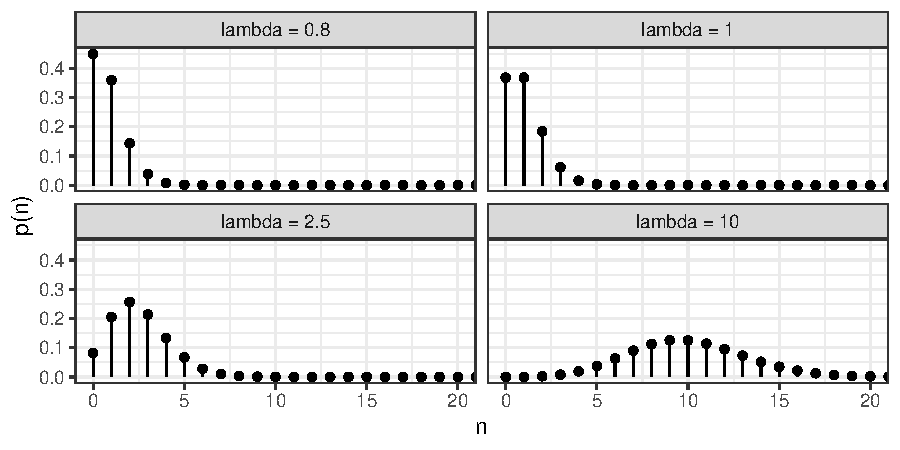
\includegraphics{_main_files/figure-latex/plot-poisson-1} 

}

\caption{Poisson distribution for some values of $\lambda$.}\label{fig:plot-poisson}
\end{figure}

The Poisson distribution is a parametric distribution that depends on only the parameter \(\lambda\). In figure \ref{fig:plot-poisson}, for different levels of \(\lambda\) the distribution is represented. These plots show how for larger values of \(\lambda\), the distribution is shifted to larger values and it is wider.

Indeed, the first two moments are:

\begin{align*}
E(N)   & = \lambda \\
Var(N) & = \lambda
\end{align*}

Thus, increasing \(\lambda\), both \(E(N)\) and \(Var(N)\) increase.

Looking to the distribution shape, we can see that:

\begin{itemize}
\tightlist
\item
  if \(\lambda<1\), the mode is in \(n=0\);
\item
  if \(\lambda=1\), \(p(0)=p(1)=\frac{1}{e}\);
\item
  if \(\lambda>1\), the mode is in a value greater than \(0\) and, as \(\lambda\) increases, the distribution assumes a bell shape similar to the Normal distribution one. The convergence to the Normal distribution can be obtained with the \emph{Central Limit Theorem}.
\end{itemize}

In non-life insurance we usually are in the case with \(\lambda<1\). E.g. the average number of claims for motor third party liability insurances in Italy, in 2018 has been 5.68\%\footnote{\href{https://www.ania.it/ricerca-avanzata/-/asset_publisher/XIyLeujL9irt/content/id/113283}{ANIA yearly statistical report for motor third party liability}}.

The property \(Var(N) = E(N)\) is an important constraint when the distribution is used in practice. It is possible that the observed data shows a different pattern. Often the observed data shows a situation where \(Var(N) > E(N)\). This phenomenon is called \emph{overdispesion}.

To address this issue it is possible to use more flexible distributions, such as Negative-Binomial distribution, or to adopt less assumptions on the response variable distribution. One common technique is the assumption of Quasi-Poisson distribution, that we will describe in chapter \ref{chap:models}.

\hypertarget{exposure}{%
\subsubsection{Exposure}\label{exposure}}

In section \ref{chap:non-life-ins} we said that non-life insurances usually have a fixed coverage period that usually spans for one year. Often we work with portfolios of insurances with different coverage periods. For example, this could be due to the presence of insurances born with shorter coverage periods or to the presence of insurances that has been closed earlier. Moreover, in companies data, often insurance data are collected for accounting years. This means that, if an insurance coverage \(c\) spans in two consecutive years \(a\) and \(a+1\), it is collected as two records: the couple \((c, a)\) and the couple \((c, a+1)\). This situation is quite common, as usually coverages start during the year and not all at the first of the year.

The coverage span for an insurance coverage is called \emph{exposure} and it is usually measured in years-at-risk. For instance, if an insurance coverage spans for 3 months, it corresponds to a quarter of year, so the exposure, measured in years-at-risk, is \(v=\frac{1}{4}\). The term year-at-risk comes from the fact that the policyholder exposure is a risk for the insurer, so the exposure is the period in which the insurer is exposed to the risk of paying claims.

It is natural to assume that, if a policyholder has a longer exposure, it is expected for him to experience more claims. Considering that we have to work with policies with different exposures, in order to take this aspect into account, the usual assumption taken in the following. Said \(M\) the number of claims the policyholder will experience during his period of exposure \(v\) and \(N\) the number of claims the policyholder would experience during one year, we assume \(E(M) = v E(N)\).

This assumption can be further extended if we assume that the claims come from a \emph{Poisson process}.

\begin{definition}[Counting Process]
\label{def:def-process-count} \iffalse (Counting Process) \fi{} A stocastic process \(\{N(t), t\ge0\}\) is called \textit{counting process} if:

\begin{enumerate}
\item The determination of N(t) are natural numbers \\
      $N(t) \in \{ 0, 1, 2, ... \} \ t\ge 0$
\item The process is not decreasing \\
      $s < t \Rightarrow N(s) \le N(t)$
\end{enumerate}
\end{definition}

In a counting process \(\{N(t), t\ge0\}\):

\begin{itemize}
\tightlist
\item
  \(N(t)\) can be interpreted as the number of events or arrivals that occur in the period \([0, t]\);
\item
  \(N(t) - N(s), \ s\le t\) can be interpreted as the number of events or arrivals that occur in the period \(]s, t]\). \(N(t) - N(s)\) is also called \emph{increment} of the process.
\end{itemize}

The counting process can be used to model the number of claims that occur to a specific policy.

\begin{definition}[Poisson Process]
\label{def:def-process-poisson} \iffalse (Poisson Process) \fi{} A counting process \(\{N(t), t\ge0\}\) is a \textit{Poisson process} with intensity \(\lambda\) if:

\begin{enumerate}
\item The increments of the process are stocastically independent \\
      $\forall n\ge0, \forall s_1 < t_1 \le \dots \le s_n < t_n$ \\
      $\Rightarrow \ N(t_1)-N(s_1), \dots, N(t_n)-N(s_n)$ are stocastically independent;
\item The probability of arrival in an interval is proportional to the size of the interval \\
      $\forall t\ge 0, \forall \Delta t >0 \ \Rightarrow \ P\left( N(t + \Delta t) - N(t) = 1 \right) = \lambda \Delta t + \omicron (\Delta t)$ \\
      where $\lim_{\Delta t \to 0}{\frac{\omicron(\Delta t)}{\Delta t}} = 0$
\item Multiple arrivals are excluded \\
      $\forall t\ge 0, \forall \Delta t >0 \ \Rightarrow \ P\left( N(t + \Delta t) - N(t) \ge 2 \right) = \omicron (\Delta t)$
\item Arrivals at time $0$ are almost impossible \\
      $P\left( N(0) = 0 \right) = 1 $
\end{enumerate}
\end{definition}

Under these hypotheses we obtain the following result:

\begin{theorem}[Poisson Process]
\label{thm:th-process-poisson} \iffalse (Poisson Process) \fi{} If \(\{N(t), t\ge 0 \}\) is a Poisson process with intensity \(\lambda\), then:

\[\forall t\ge 0, \forall \Delta t >0, \ \Rightarrow \ N(t + \Delta t) - N(t) \sim Poisson(\lambda \Delta t)\]
\end{theorem}

This result tells us that the distribution of the number of events in any interval \(]t, t+\Delta t]\) only depends on the size of the interval \(\Delta t\). Moreover, for the Poisson property we saw in section \ref{chap:dist-n}, we get:

\[E(N(t + \Delta t) - N(t)) = \lambda \Delta t\]

So, the expected number of arrivals is proportional to the size of the interval \(\Delta t\). The intensity of the process \(\lambda\) can be also interpreted as the expected number of claims in a unitary period.

If we assume that the claims that occur to a policy comes from a Poisson process with intensity \(\lambda\), if we observe that policy for the period \(]t, t+v]\), the claims count in that exposure period \(M\) are distributed as:

\[ M\sim Poisson(\lambda \Delta t) \]

In particular, if the observed period spans 1 year, we get:

\[ M = N \sim Poisson(\lambda) \]

\hypertarget{distribution-for-the-claims-size-z}{%
\subsubsection{\texorpdfstring{Distribution for the claims size \(Z\)}{Distribution for the claims size Z}}\label{distribution-for-the-claims-size-z}}

The claim size \(Z\) is a continuour variable with determination in \([0, +\infty[\). As for the claims count \(N\), even if in practice it can't be arbitrarily high, it is usually modeled with distributions that give a positive probability to all the numbers in \(]0, +\infty[\). As the null claims are excluded, it is natural tu assume \(P\left( Z=0 \right) = 0\). One of the most common distribution used for \(Z\) is the Gamma distribution.

\begin{definition}[Gamma Distribution]
\label{def:def-gamma} \iffalse (Gamma Distribution) \fi{} A random variable \(Z\) with support \([0, +\infty[\) has a Gamma distribution, if its probability density function is:
\[
f_Z(z) = \frac{\rho^\alpha}{\Gamma(\alpha)}z^{\alpha-1}e^{-\rho z}, \quad \alpha > 0, \ \rho > 0
\]
where \(\Gamma(\alpha) = \int_{0}^{+\infty}{z^{\alpha - 1} e^{-z} \mathrm{d} z}\)

We will indicate it with the notation \(Z \sim Gamma(\alpha, \rho)\).
\end{definition}

\begin{figure}[hbtp]

{\centering 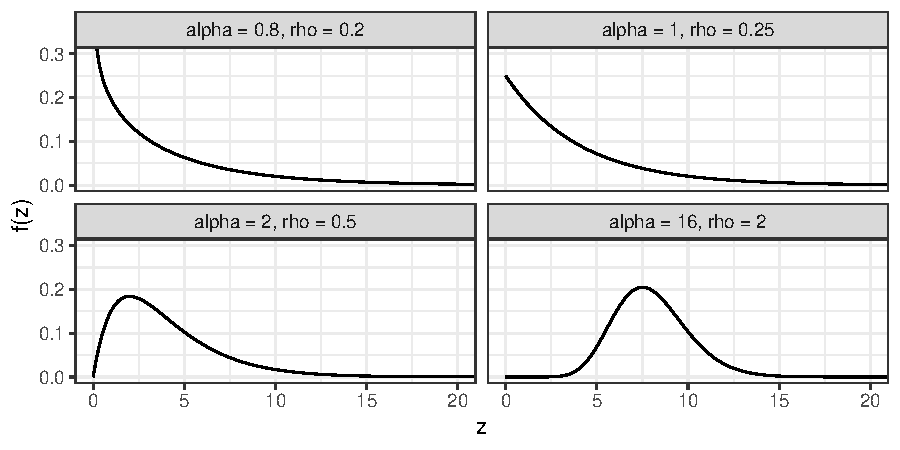
\includegraphics{_main_files/figure-latex/plot-gamma-1} 

}

\caption{Gamma distribution for some values of $\alpha$ and $\rho$.}\label{fig:plot-gamma}
\end{figure}

The Gamma distribution is a parametric distribution that depends on two parameters:

\begin{itemize}
\tightlist
\item
  \(\alpha > 0\), called shape parameter
\item
  \(\rho > 0\), called scale parameter
\end{itemize}

The first two moments of the Gamma distribution are:

\begin{align*}
E(Z)   & = \frac{\alpha}{\rho} \\
Var(Z) & = \frac{\alpha}{\rho^2}
\end{align*}

In figure \ref{fig:plot-gamma}, for different levels of \(\alpha\) and \(\gamma\) the distribution is represented. These plots show how changing the values of \(\alpha\) and \(\gamma\), the shape changes. We can see that:

\begin{itemize}
\tightlist
\item
  if \(\alpha < 1\), \(f_z(\cdot)\) is not defined in \(0\) and it has a vertical asymptote in \(z = 0\). In \(]0, +\infty]\) it is monotonically decreasing.
\item
  if \(\alpha = 1\), \(f_z(\cdot)\) starts from \(f(0) = \rho\) and then decreases monotonically. In this case, the density function becomes \(f_z(z) = \rho e^{-\rho z}\) and the distribution is also called exponential distribution.
\item
  if \(\alpha > 0\), \(f_z(\cdot)\) starts from \(f(0) = 0\), increases until the mode and then decreases.
\end{itemize}

In figure \ref{fig:plot-gamma} the first three distributions represented have the same expected value \(E(Z)=\frac{\alpha}{\rho} = 4\), but different shapes. The third and the fourth have the same variance \(Var(Z) = \frac{\alpha}{\rho^2} = 8\), but different expected values. As the shape parameter \(\alpha\) increases, the distribution assumes a bell shape similar to the Normal distribution one. The convergence to the Normal distribution can be obtained with the \emph{Central Limit Theorem}.

From the parametrical form of the moments, we get that \(Var(Z)\) and \(E(Z)\) are linked as follows:

\[Var(Z) = \frac{\alpha}{\rho^2} = \frac{1}{\alpha} \left(E(Z) \right)^ 2\]

From this relation we find that the coefficient of variation is:
\[CV(Z) = \frac{\sqrt{Var(Z)}}{E(Z)} = \frac{1}{\sqrt{\alpha}}\]

This result means that, given the shape parameter \(\alpha\), the coefficient of variation is constant. As we saw for Poisson distribution, it is possible that observed data shows a different pattern.

Another characteristic of Gamma distribution that could be problematic in modeling claims size is that it has a light tail. This means that, as \(z\) goes to \(+\infty\), \(f_Z(z)\) aproaches \(0\) quite fast. This could lead to a poor fitting for \emph{large claims}. Other distributions with havier tails are for example the \emph{log-Normal} and the \emph{Pareto}.

\hypertarget{chap:large-claims}{%
\subsubsection{Large claims}\label{chap:large-claims}}

Modeling large claims in quite difficult in practice because usually there is not a lot of observed data on them, so it is hard to understand if they are related to some risk factors (identifiable by the pricing variables) or they happen just by chance.

First of all, to model large claims, we must define what a large claim is. What is usually done in practice is just choosing a threshold \(\bar{z}\) and considering large all the claims with a size that exceeds that threshold. The value \(\bar{z}\) must be chosen sufficiently big to consider large the claims above \(\bar{z}\), but not so big that there are not enough observed claims that exceeds \(\bar{z}\). One common choice for Motor Third Party Liability in European markets could be \(\bar{z} = 100' 000 \text{\euro}\).

\begin{definition}[Large and Attritional Claims]
\label{def:def-large-claim} \iffalse (Large and Attritional Claims) \fi{} Given a predetermined threshold \(\bar{z}\), we say that:

\begin{itemize}
\item a claim $Z$ is a \textit{large claim} if $Z > \bar{z}$
\item a claim $Z$ is an \textit{attritional claim} if $Z \le \bar{z}$
\end{itemize}

For each claim \(Z\) we call:

\begin{itemize}
\item \textit{Capped Claim Size} \\
      $Z' = \min(Z, \bar{z})$;
\item \textit{Excess Over the Threshold} \\
      $Z'' = \max(Z - \bar{z}, 0)$.
\end{itemize}
\end{definition}

In figure \ref{fig:large-claim} the \emph{Capped Claim Size} and the \emph{Excess Over the Threshold} are shown. It is easy to show that \(Z\) can be decomposed as:
\[Z = Z' + Z''\]

\begin{figure}
\centering
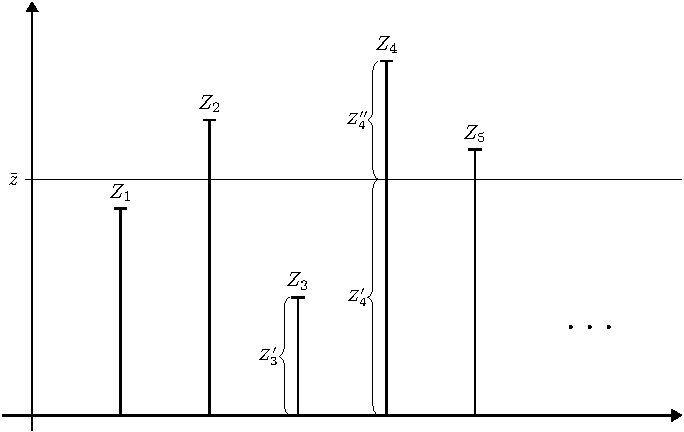
\includegraphics{_main_files/figure-latex/large-claim-1.pdf}
\caption{\label{fig:large-claim}Large claims.}
\end{figure}

Given the total number of claims \(N\), it can be decomposed as:
\[N = N^{(a)} + N^{(l)}\]

where

\begin{itemize}
\tightlist
\item
  \(N^{(a)}\) is the attritional claims count, i.e.~the number of claims with size \(Z \le \bar{z}\);
\item
  \(N^{(l)}\) is the large claims count, i.e.~the number of claims with size \(Z > \bar{z}\);
\end{itemize}

Let's indicate with \(Z_{(i)}\) the \(i\)\textsuperscript{th} in order from the smallest to the bigger. Sorting the claims we can separate the attritional claims from the large claims as follows:

\[
\underbrace{Z_{(1)}, Z_{(2)}, \dots, Z_{(N^{(a)})}}_{\text{Attritional Claims}},
\underbrace{Z_{(N^{(a)} + 1)}, Z_{(N^{(a)} + 2)}, \dots Z_{(N^{(a)} + N^{(l)})}}_{\text{Large Claims}}
\]

In order to model the large claims it is possible to use the following three decompositions of the total cost of claims \(S\):

\begin{eqnarray}
  \nonumber
  S & = & \underbrace{Z_{(1)} + Z_{(2)} + \dots + Z_{(N^{(a)})}}_{\text{Attritional Claims}} +
        \underbrace{Z_{(N^{(a)} + 1)} + Z_{(N^{(a)} + 2)} + \dots Z_{(N^{(a)} + N^{(l)})}}_{\text{Large Claims}} \\
  \label{large-claim-decomposition-1}
    & = & \underbrace{\sum_{i=1}^{N^{(a)}}{Z_{(i)}}}_{=S^{(a)}} +
            \underbrace{\sum_{i = N^{(a)} + 1}^{N^{(a)} + N^{(l)}}{Z_{(i)}}}_{=S^{(l)}}
    \ = \ S^{(a)} + S^{(l)} \\[12pt]
  \label{large-claim-decomposition-2}
  S & = & \sum_{i=1}^{N}{Z_i}
    \ = \ \sum_{i=1}^{N}{\left(
      \{Z_i|Z_i>\bar{z}\} I_{Z_i>\bar{z}} +
      \{Z_i|Z_i\le\bar{z}\} I_{Z_i\le\bar{z}}
      \right)} \\[12pt]
  \label{large-claim-decomposition-3}
  S & = & \sum_{i=1}^{N}{Z_i}
    \ = \ \sum_{i=1}^{N}{\left(Z'_i + Z''_i\right)}
    \ = \ \sum_{i=1}^{N}{\left(Z'_i + Z''_i I_{Z_i > \bar{z}}\right)}
\end{eqnarray}

These three decompositions of \(S\) are useful because they provide three decompositions of \(E(S)\):

\begin{eqnarray}
  \nonumber
  E(S) & = & E(S^{(a)}) + E(S^{(l)}) \\
    \label{large-claim-decomposition-expected-1}
    & = & E(N^{(a)}) E(Z|Z\le\bar{z}) + E(N^{(l)}) E(Z|Z>\bar{z}) \\[12pt]
  \nonumber
  E(S) & = & E(N) E(Z) \\
    \nonumber
    & = & E(N) \left[P(Z\le\bar{z}) E(Z|Z\le\bar{z}) + P(Z>\bar{z}) E(Z|Z > \bar{z}) \right] \\
    \label{large-claim-decomposition-expected-2}
    & = & E(N) \left[\left( 1 - P(Z>\bar{z}) \right) E(Z|Z\le\bar{z}) + P(Z>\bar{z}) E(Z|Z > \bar{z})\right] \\[12pt]
  \nonumber
  E(S) & = & E(N) E(Z) \\
    \label{large-claim-decomposition-expected-3}
    & = & E(N) \left[E(Z') + P(Z>\bar{z}) E(Z'')\right]
\end{eqnarray}

\ref{large-claim-decomposition-expected-1}, \ref{large-claim-decomposition-expected-2} and \ref{large-claim-decomposition-expected-3} provide three approaches to model attritional and large claims.

\begin{enumerate}
\def\labelenumi{\arabic{enumi}.}
\tightlist
\item
  Looking to \ref{large-claim-decomposition-expected-1} we can model separately attritional claims and large claims. Modeling \(N^{(a)}\) and \(Z|Z\le\bar{z}\) we estimate the total cost of claims for the attritional part \(S^{(a)}\); modeling \(N^{(l)}\) and \(Z|Z>\bar{z}\) we estimate the total cost of claims for the large part \(S^{(l)}\).
\item
  Looking to \ref{large-claim-decomposition-expected-2} we can model together the claim count \(N\), and then we can model the cost of the attritional claims \(Z|Z\le\bar{z}\), the cost of the large claims \(Z|Z>\bar{z}\) and the probability to exceed the threshold \(P(Z>\bar{z})\).
\item
  Looking to \ref{large-claim-decomposition-expected-3} we can model together the claim count \(N\), and then we can model the capped claims size \(Z'\), the excess over the threshold \(Z''\) and the probability to exceed the threshold \(P(Z>\bar{z})\).
\end{enumerate}

If the large claims component weights a lot on the total cost of claims, these approaches could lead to quite different estimations of \(E(S)\). In particular, if in the observed data the number of large claims is small, it will be hard to model both \(N^{(l)}\) and \(P(Z>\bar{z})\), so the modeling process could lead to a flat or almost flat model for these components. However, with the first approach, a flat model for \(N^{(l)}\) leads to distribute the observed total cost of large claims proportionally to all the policies, while with the second and the third, a flat model for \(P(Z>\bar{z})\) leads to distribute the observed total cost of large claims proportionally to the expected number of claims \(E(N)\). So, with the first approach, a flat model brings to more solidarity between policies, while, with the second approach, a flat model could bring to an exacerbation of the differences identified by modeling \(N\).

For the second approach we must also introduce a distribution suitable for modeling \(P(Z>\bar{z})\).

\hypertarget{binomial-distribution}{%
\subsubsection{Binomial distribution}\label{binomial-distribution}}

The \emph{binomial distribution} is used to model the counting on events that occurs (successes) in a fixed amount of trials \(n\). For example we can use it to model the number of large claims withing a fixed number of \(n\) claims.

\begin{definition}[Binomial Distribution]
\label{def:def-binomial} \iffalse (Binomial Distribution) \fi{} A random variable \(Y\) with support \(\{0,1,2, \dots, n \}\) has a Binomial distribution, if its probability function is:

\[
p_Y(y) = P\left( Y = y \right) = \binom{n}{y} p^y (1-p)^{n-y}, \quad p \in [0, 1]
\]

We will indicate it with the notation \(Y \sim Binomial(n, p)\).
\end{definition}

\begin{figure}[hbtp]

{\centering 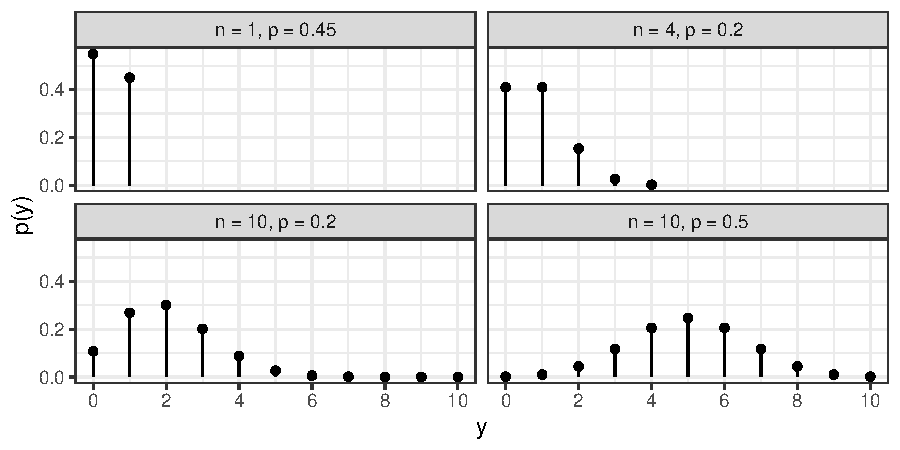
\includegraphics{_main_files/figure-latex/plot-binomial-1} 

}

\caption{Binomial distribution for some values of $n$ and $p$.}\label{fig:plot-binomial}
\end{figure}

The binomial distribution is a parametric distribution that depends on the parameters \(n\) and \(p\). \(n\) represents the number of trials, while \(p\) represents the probability for a trial to success. The assumption is that the \(n\) trials are identical, so they have all the same probability \(p\) to success. In figure \ref{fig:plot-binomial}, for different levels of \(n\) and \(p\), the distribution is represented.

The first two moments of the binomial distribution are:

\begin{align*}
E(N)   & = np \\
Var(N) & = np(1-p)
\end{align*}

If \(n = 1\), the binomial distribution assumes only the values \(1\) (with probability \(p\)) and \(0\) (with probability \(1-p\)). In this case it is also called \emph{Bernoullian distribution} and it can be used to model the indicator of an event \(I_E\).

If \(n>1\), the binomial distribution assumes a shape centered on its expected value \(E(Y)=np\) and fading for values of \(y\) that moves away from \(E(Y)\). As \(n\) increases, the distribution assumes a bell shape similar to the Normal distribution one. The convergence to the Normal distribution can be obtained with the \emph{Central Limit Theorem}.

In non-life insurance pricing, the binomial distribution can be used to model the probability for a claim to have specific characteristics. For example we can use it to model the probability that a certain claim is a large one \(P(Z>\bar{z})\) in order to model separately attritional claims severity \(\{Z|Z\le\bar{z}\}\) and large claims severity \(\{Z|Z>\bar{z}\}\), as we have seen in section section \ref{chap:large-claims}.

Another example is the decomposition between claims with only damage to things and claims with also injuries to people. Modeling separately these two components is useful because they usually have a different distribution for the claim size.

As for large claims we can decompose \(S\) in the following two ways:

\begin{eqnarray}
  \nonumber
  E(S) & = & E(S^{(things)}) + E(S^{(inj)}) \\
    \label{inj-claim-decomposition-expected-1}
    & = & E(N^{(things)}) E(Z|\bar{J}) + E(N^{(inj)}) E(Z|J) \\[12pt]
  \nonumber
  E(S) & = & E(N) E(Z) \\
    \nonumber
    & = & E(N) \left[P(\bar{J}) E(Z|\bar{J}) + P(J) E(Z|J) \right] \\
    \label{inj-claim-decomposition-expected-2}
    & = & E(N) \left[\left( 1 - P(J) \right) E(Z|\bar{J}) + P(J) E(Z|J)\right]
\end{eqnarray}

where:

\begin{itemize}
\tightlist
\item
  \(N^{(things)}\) is the number of claims with only damage to things;
\item
  \(N^{(inj)}\) is the number of claims with injuries;
\item
  \(J\) is the event that represent that a specific claim presents injuries; such as \(Z\) is a representative for \(Z_1, Z_2, \dots, Z_N\), \(J\) is a representative for \(J_1, J_2, \dots, J_N\).
\end{itemize}

Combining this decomposition with what we have seen in large claims decomposition, we can further develop our decomposition taking into account both the presence or absence of injuries and the occurrence or not of a large claim. One example could be:

\begin{align*}
E(S) & = E(N) \left[\left( 1 - P(J) \right) E(Z|\bar{J}) + P(J) E(Z|J) \right] \\[11pt]
  & = E(N) \left\{ \right. \\
  & \qquad \left( 1 - P(J) \right) E(Z|\bar{J}) \\
  & \qquad + P(J) \left[ \right. \\
  & \qquad \qquad P(Z \le \bar{z} | J) E\left( Z \mid Z\le \bar{z} \land J \right) \\
  & \qquad \qquad + P(Z < \bar{z} | J) E\left( Z \mid Z < \bar{z} \land J \right) \\
  & \qquad \left. \right] \\
  & \quad \left. \right\}
\end{align*}

This way, we are decomposing only the claims with injuries between attritional and large. That makes sense because claims that don't produce injuries usually have small severities.

\hypertarget{model-fitting-and-data-available}{%
\subsection{Model fitting and data available}\label{model-fitting-and-data-available}}

Once we have chosen how to decompose \(S\), we have to model the response variables needed for that decomposition (\(N\), \(Z\), \(I_J\), \ldots) with the explanatory variables. Thus we have to estimate a function \(r:\mathcal{X}\rightarrow \mathcal{C}\) as defined in \ref{def:modeling}.

In order to estimate \(r(\cdot)\) we have also to take some assumptions on the distribution of the response variable and on the shape of \(r(\cdot)\). We will call \emph{model} a set of assumptions on the response variable and on the shape of \(r(\cdot)\). We will discuss some of the most widespread models for claims count and claims severity in chapter \ref{chap:models}.

Defined the model, we have to estimate it using observed data. In general, to model a response variable \(Y_i\) with the explanatory variables \(\boldsymbol{x}_i=(x_{i1}, x_{i2}, \dots, x_{ip})\in \mathcal{X} \subseteq \mathbb{R}^p\), the observed data is in the form:

\[
(\boldsymbol{x}_1, w_1, y_1), \ (\boldsymbol{x}_2, w_2, y_2), \ \dots, \ (\boldsymbol{x}_i, w_i, y_i), \ \dots, \ (\boldsymbol{x}_n, w_n, y_n)
\]
where:

\begin{itemize}
\tightlist
\item
  \(n\) is the number of observations in the dataset;
\item
  \(\boldsymbol{x}_i\in \mathcal{X} \subseteq \mathbb{R}^p\) is the set of explanatory variable for the observation \(i\);
\item
  \(w_i\) is the weight for the observation \(i\);
\item
  \(y_i\in \mathcal{Y}\ \subseteq \mathbb{R}\) is the realization of the response variable \(Y_i\) for the observation \(i\).
\end{itemize}

What an observation is, depends on the variable we are modeling. For instance:

\begin{itemize}
\tightlist
\item
  If we are modeling the yearly claim count \(N_i\), each observation could be a policy (or a couple (policy, accounting year)), the weights could be the exposures \(v_i\) and the realizations of response variables could be the number of observed claims for that policy (or couple (policy, accounting year)).
\item
  If we are modeling the claim severity \(Z_j\), each observation could be a claim \(j\), the weights could all be \(1\) and the realizations of response variables could be the observed cost for the claim \(j\). It is also possible to model the claim severity taking into account the total cost of claims for the policy \(S_i = \sum_{j=1}^{N_i}{Z_j}\). In this case, each observation would be a policy \(i\), the weights would be the number of claims for each policy \(n_i\) and the realizations of response variables would be the total observed cost for the claims of the policy \(i\).
\item
  If we are modeling the occurrence of injuries in a claim \(I_{Jj}\), each observation could be a claim \(j\), the weights could be all \(1\) and the realizations of response variables could be an indicator that assume the value \(1\) if the claim \(j\) caused injuries and \(0\) otherwise. As for the claim severity, we can also aggregate data for policy, so each observation would be a policy \(i\), the weights would be the number of claims \(n_i\) for the policy \(i\) and the realizations of response variables would be the number of claims that caused injuries among the claims of the policy \(i\).
\end{itemize}

In each of these cases, \(y_i\) is seen as a realization of the random variable \(Y_i\). With an inferential process we obtain estimations on \(Y_i\) based on observations of their realizations \(y_i\).

\hypertarget{settlement-process-and-ibnr}{%
\subsubsection{Settlement process and IBNR}\label{settlement-process-and-ibnr}}

One of the challenges in non-life insurance pricing is that obtaining the observed data is not so straightforward. In many insurance coverages, the settlement process could last many years, so, if we want to develop models using data from recent years, not all the information is available. To better understand this aspect we have to discuss how the settlement process works.

In figure \ref{fig:settlement-process} the settlement process for a claim is represented. At time \(t_1\) the insured event (e.g.~an accident) occurs. From this moment a liability for the insurer emerges, even if the insurer has not been notified yet. This liability is called \emph{Outstanding Loss Liability}. In \(t_2\) the claim in reported and the insurance is notified about the occurrence of the event. From this moment the settlement process starts. This process consists in evaluating the event and understanding the responsibilities and the entity of the damage. During this process, controversies between the parts can emerge and, in particular if injuries occurred, the damage evaluation can takes a lot of time. When the situation in clear and everything is defined, the claim is settled and the liabilities are payed. In \(t_3\) we have the settlement and in \(t_4\) the claim is closed. In is possible that \(t_4=t_3\), but in general it is not always the case. If the settlement process takes a long time and the insurer already knows he will have to pay something, he can pay some partial payments during the period \([t_2, t_3]\). These intermediate payments are payed in the times \(\tau_1, \tau_2, \dots, \tau_n \in [t_2, t_3]\). It is also possible that a claim is opened and then get closed without any payment. After the closing (\(t_4\)) it is also possible that a claim is reopened and that more payments emerge.

\begin{figure}
\centering
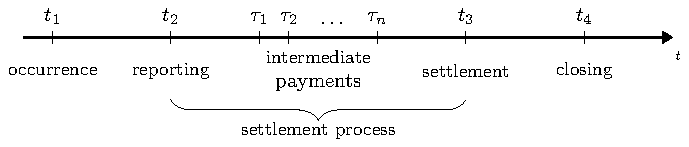
\includegraphics{_main_files/figure-latex/settlement-process-1.pdf}
\caption{\label{fig:settlement-process}Claim timeline.}
\end{figure}

From the moment the claim is reported (\(t_2\)), the insurer estimates how much he is going to pay for that claim and he allocates that sum in a reserve. As new information emerges and some payments are settled, the reserve is updated. The aim for this reserve is to have a best estimate for the future payments for the claims already emerged. As the claim is settled, the sum between the payed and the reserved converges to the final cost of the claim.

From this description emerges that:

\begin{itemize}
\tightlist
\item
  In the period \(]t_1, t_2[\) the insurer have an outstanding loss liability for an event that has not been reported yet; in this case we will talk about \emph{Incurred But Not Yet Reported} (\emph{IBNyR}) claims.
\item
  In the period \([t_2, t_3[\) the insurer have an outstanding loss liability for an event that has been reported, but has not been totally settled yet, so that liability is just an estimate; in this case we will talk about \emph{Incurred But Not Enough Reported} (\emph{IBNeR}) claims.
\end{itemize}

This issue is particularly challenging when we have to perform a risk evaluation at a specific time. In general \(t_1, t_2,\dots\) are not known a priori, so we don't know if in the future more claims for accidents occurred in the past will be reported and we don't know if the ones that are already reported will experience a revaluation. That means that, in general, when we model \(N\) and \(Z\) at a specific time \(t\), we can't observe the total number of claims occurred to each policy \(n_i\) and the payments for each claim \(z_j\). What we can use is:

\begin{itemize}
\tightlist
\item
  the number of reported claims \(n_i^{(t)} = n_i^{(\text{reported in } t)}\)
\item
  the sums already payed for each claim \(z_j^{(\text{payed in }t)}\) and the sums reserved for each claim \(z_j^{(\text{reserved in } t)}\): \(z_j^{(t)} = z_j^{(\text{payed in }t)} + z_j^{(\text{reserved in } t)}\)
\end{itemize}

When we use these variables for modeling the total cost of claims we must be particularly aware on what we are using. In general

\begin{align*}
n_i & \ne n_i^{(t))} \\
z_j & \ne z_j^{(t)}
\end{align*}

\hypertarget{commercial-tariff-and-offer-price}{%
\section{Commercial Tariff and Offer Price}\label{commercial-tariff-and-offer-price}}

\newpage

\hypertarget{non-life-insurance-in-italy}{%
\section{Non-Life Insurance in Italy}\label{non-life-insurance-in-italy}}

Lorem ipsum dolor sit amet, consectetur adipiscing elit. Vivamus id mauris interdum, malesuada ante eu, tempus lacus. Aliquam blandit tortor a velit ultricies, eget pharetra nulla egestas. Suspendisse pellentesque finibus est, vitae ullamcorper magna convallis ut. Nulla a lectus in ligula iaculis convallis. Pellentesque tortor mauris, tempor nec dictum et, facilisis sit amet dolor. Mauris nibh quam, molestie non ex quis, hendrerit dignissim nulla. Aliquam sit amet dui at diam vestibulum malesuada a id lacus. Phasellus viverra orci vitae sem pretium, eu consequat libero euismod.

Cras suscipit aliquam consequat. Quisque sodales lacus ac erat malesuada, eu laoreet enim vestibulum. Sed id ante id ligula auctor ullamcorper. Sed luctus rutrum mollis. Vestibulum sed ultrices quam. Duis id orci ut enim elementum maximus id quis justo. Pellentesque rutrum ligula in aliquam rhoncus. Integer suscipit nisl at mi efficitur interdum. Aenean et orci elit.

Nam ultricies est et iaculis tempus. Quisque leo lorem, sagittis et ligula a, blandit mattis velit. Phasellus pretium, orci et semper finibus, dui nulla tempor nisl, vel vehicula magna diam nec sem. Praesent finibus commodo enim non laoreet. Lorem ipsum dolor sit amet, consectetur adipiscing elit. Curabitur ut pellentesque purus. Proin hendrerit, odio vel sodales porta, ex lorem feugiat sem, non fringilla libero ex ac ligula. Quisque facilisis eros at suscipit rhoncus.

\hypertarget{the-actuary-role}{%
\section{The actuary role}\label{the-actuary-role}}

Lorem ipsum dolor sit amet, consectetur adipiscing elit. Vivamus id mauris interdum, malesuada ante eu, tempus lacus. Aliquam blandit tortor a velit ultricies, eget pharetra nulla egestas. Suspendisse pellentesque finibus est, vitae ullamcorper magna convallis ut. Nulla a lectus in ligula iaculis convallis. Pellentesque tortor mauris, tempor nec dictum et, facilisis sit amet dolor. Mauris nibh quam, molestie non ex quis, hendrerit dignissim nulla. Aliquam sit amet dui at diam vestibulum malesuada a id lacus. Phasellus viverra orci vitae sem pretium, eu consequat libero euismod.

Cras suscipit aliquam consequat. Quisque sodales lacus ac erat malesuada, eu laoreet enim vestibulum. Sed id ante id ligula auctor ullamcorper. Sed luctus rutrum mollis. Vestibulum sed ultrices quam. Duis id orci ut enim elementum maximus id quis justo. Pellentesque rutrum ligula in aliquam rhoncus. Integer suscipit nisl at mi efficitur interdum. Aenean et orci elit.

Nam ultricies est et iaculis tempus. Quisque leo lorem, sagittis et ligula a, blandit mattis velit. Phasellus pretium, orci et semper finibus, dui nulla tempor nisl, vel vehicula magna diam nec sem. Praesent finibus commodo enim non laoreet. Lorem ipsum dolor sit amet, consectetur adipiscing elit. Curabitur ut pellentesque purus. Proin hendrerit, odio vel sodales porta, ex lorem feugiat sem, non fringilla libero ex ac ligula. Quisque facilisis eros at suscipit rhoncus.

Questa è una citazione \autocite{Shea2014,Lottridge2012}

--\textgreater{}

\hypertarget{chap:models}{%
\chapter{\texorpdfstring{\textbf{Statistical models for Non Life Insurance Pricing}}{Statistical models for Non Life Insurance Pricing}}\label{chap:models}}

\minitoc  

\chaptermark{Statistical models for Non Life Insurance Pricing}

\hypertarget{statistical-models}{%
\section{Statistical Models}\label{statistical-models}}

Lorem ipsum dolor sit amet, consectetur adipiscing elit. Vivamus id mauris interdum, malesuada ante eu, tempus lacus. Aliquam blandit tortor a velit ultricies, eget pharetra nulla egestas. Suspendisse pellentesque finibus est, vitae ullamcorper magna convallis ut. Nulla a lectus in ligula iaculis convallis. Pellentesque tortor mauris, tempor nec dictum et, facilisis sit amet dolor. Mauris nibh quam, molestie non ex quis, hendrerit dignissim nulla. Aliquam sit amet dui at diam vestibulum malesuada a id lacus. Phasellus viverra orci vitae sem pretium, eu consequat libero euismod.

Cras suscipit aliquam consequat. Quisque sodales lacus ac erat malesuada, eu laoreet enim vestibulum. Sed id ante id ligula auctor ullamcorper. Sed luctus rutrum mollis. Vestibulum sed ultrices quam. Duis id orci ut enim elementum maximus id quis justo. Pellentesque rutrum ligula in aliquam rhoncus. Integer suscipit nisl at mi efficitur interdum. Aenean et orci elit.

Nam ultricies est et iaculis tempus. Quisque leo lorem, sagittis et ligula a, blandit mattis velit. Phasellus pretium, orci et semper finibus, dui nulla tempor nisl, vel vehicula magna diam nec sem. Praesent finibus commodo enim non laoreet. Lorem ipsum dolor sit amet, consectetur adipiscing elit. Curabitur ut pellentesque purus. Proin hendrerit, odio vel sodales porta, ex lorem feugiat sem, non fringilla libero ex ac ligula. Quisque facilisis eros at suscipit rhoncus.

\hypertarget{glm}{%
\subsection{GLM}\label{glm}}

Lorem ipsum dolor sit amet, consectetur adipiscing elit. Vivamus id mauris interdum, malesuada ante eu, tempus lacus. Aliquam blandit tortor a velit ultricies, eget pharetra nulla egestas. Suspendisse pellentesque finibus est, vitae ullamcorper magna convallis ut. Nulla a lectus in ligula iaculis convallis. Pellentesque tortor mauris, tempor nec dictum et, facilisis sit amet dolor. Mauris nibh quam, molestie non ex quis, hendrerit dignissim nulla. Aliquam sit amet dui at diam vestibulum malesuada a id lacus. Phasellus viverra orci vitae sem pretium, eu consequat libero euismod.

Cras suscipit aliquam consequat. Quisque sodales lacus ac erat malesuada, eu laoreet enim vestibulum. Sed id ante id ligula auctor ullamcorper. Sed luctus rutrum mollis. Vestibulum sed ultrices quam. Duis id orci ut enim elementum maximus id quis justo. Pellentesque rutrum ligula in aliquam rhoncus. Integer suscipit nisl at mi efficitur interdum. Aenean et orci elit.

Nam ultricies est et iaculis tempus. Quisque leo lorem, sagittis et ligula a, blandit mattis velit. Phasellus pretium, orci et semper finibus, dui nulla tempor nisl, vel vehicula magna diam nec sem. Praesent finibus commodo enim non laoreet. Lorem ipsum dolor sit amet, consectetur adipiscing elit. Curabitur ut pellentesque purus. Proin hendrerit, odio vel sodales porta, ex lorem feugiat sem, non fringilla libero ex ac ligula. Quisque facilisis eros at suscipit rhoncus.

\hypertarget{elastic-net}{%
\subsection{Elastic Net}\label{elastic-net}}

Lorem ipsum dolor sit amet, consectetur adipiscing elit. Vivamus id mauris interdum, malesuada ante eu, tempus lacus. Aliquam blandit tortor a velit ultricies, eget pharetra nulla egestas. Suspendisse pellentesque finibus est, vitae ullamcorper magna convallis ut. Nulla a lectus in ligula iaculis convallis. Pellentesque tortor mauris, tempor nec dictum et, facilisis sit amet dolor. Mauris nibh quam, molestie non ex quis, hendrerit dignissim nulla. Aliquam sit amet dui at diam vestibulum malesuada a id lacus. Phasellus viverra orci vitae sem pretium, eu consequat libero euismod.

Cras suscipit aliquam consequat. Quisque sodales lacus ac erat malesuada, eu laoreet enim vestibulum. Sed id ante id ligula auctor ullamcorper. Sed luctus rutrum mollis. Vestibulum sed ultrices quam. Duis id orci ut enim elementum maximus id quis justo. Pellentesque rutrum ligula in aliquam rhoncus. Integer suscipit nisl at mi efficitur interdum. Aenean et orci elit.

Nam ultricies est et iaculis tempus. Quisque leo lorem, sagittis et ligula a, blandit mattis velit. Phasellus pretium, orci et semper finibus, dui nulla tempor nisl, vel vehicula magna diam nec sem. Praesent finibus commodo enim non laoreet. Lorem ipsum dolor sit amet, consectetur adipiscing elit. Curabitur ut pellentesque purus. Proin hendrerit, odio vel sodales porta, ex lorem feugiat sem, non fringilla libero ex ac ligula. Quisque facilisis eros at suscipit rhoncus.

\hypertarget{gam}{%
\subsection{GAM}\label{gam}}

Lorem ipsum dolor sit amet, consectetur adipiscing elit. Vivamus id mauris interdum, malesuada ante eu, tempus lacus. Aliquam blandit tortor a velit ultricies, eget pharetra nulla egestas. Suspendisse pellentesque finibus est, vitae ullamcorper magna convallis ut. Nulla a lectus in ligula iaculis convallis. Pellentesque tortor mauris, tempor nec dictum et, facilisis sit amet dolor. Mauris nibh quam, molestie non ex quis, hendrerit dignissim nulla. Aliquam sit amet dui at diam vestibulum malesuada a id lacus. Phasellus viverra orci vitae sem pretium, eu consequat libero euismod.

Cras suscipit aliquam consequat. Quisque sodales lacus ac erat malesuada, eu laoreet enim vestibulum. Sed id ante id ligula auctor ullamcorper. Sed luctus rutrum mollis. Vestibulum sed ultrices quam. Duis id orci ut enim elementum maximus id quis justo. Pellentesque rutrum ligula in aliquam rhoncus. Integer suscipit nisl at mi efficitur interdum. Aenean et orci elit.

Nam ultricies est et iaculis tempus. Quisque leo lorem, sagittis et ligula a, blandit mattis velit. Phasellus pretium, orci et semper finibus, dui nulla tempor nisl, vel vehicula magna diam nec sem. Praesent finibus commodo enim non laoreet. Lorem ipsum dolor sit amet, consectetur adipiscing elit. Curabitur ut pellentesque purus. Proin hendrerit, odio vel sodales porta, ex lorem feugiat sem, non fringilla libero ex ac ligula. Quisque facilisis eros at suscipit rhoncus.

\hypertarget{gbm}{%
\subsection{GBM}\label{gbm}}

Lorem ipsum dolor sit amet, consectetur adipiscing elit. Vivamus id mauris interdum, malesuada ante eu, tempus lacus. Aliquam blandit tortor a velit ultricies, eget pharetra nulla egestas. Suspendisse pellentesque finibus est, vitae ullamcorper magna convallis ut. Nulla a lectus in ligula iaculis convallis. Pellentesque tortor mauris, tempor nec dictum et, facilisis sit amet dolor. Mauris nibh quam, molestie non ex quis, hendrerit dignissim nulla. Aliquam sit amet dui at diam vestibulum malesuada a id lacus. Phasellus viverra orci vitae sem pretium, eu consequat libero euismod.

Cras suscipit aliquam consequat. Quisque sodales lacus ac erat malesuada, eu laoreet enim vestibulum. Sed id ante id ligula auctor ullamcorper. Sed luctus rutrum mollis. Vestibulum sed ultrices quam. Duis id orci ut enim elementum maximus id quis justo. Pellentesque rutrum ligula in aliquam rhoncus. Integer suscipit nisl at mi efficitur interdum. Aenean et orci elit.

Nam ultricies est et iaculis tempus. Quisque leo lorem, sagittis et ligula a, blandit mattis velit. Phasellus pretium, orci et semper finibus, dui nulla tempor nisl, vel vehicula magna diam nec sem. Praesent finibus commodo enim non laoreet. Lorem ipsum dolor sit amet, consectetur adipiscing elit. Curabitur ut pellentesque purus. Proin hendrerit, odio vel sodales porta, ex lorem feugiat sem, non fringilla libero ex ac ligula. Quisque facilisis eros at suscipit rhoncus.

\hypertarget{model-comparison}{%
\section{Model comparison}\label{model-comparison}}

Lorem ipsum dolor sit amet, consectetur adipiscing elit. Vivamus id mauris interdum, malesuada ante eu, tempus lacus. Aliquam blandit tortor a velit ultricies, eget pharetra nulla egestas. Suspendisse pellentesque finibus est, vitae ullamcorper magna convallis ut. Nulla a lectus in ligula iaculis convallis. Pellentesque tortor mauris, tempor nec dictum et, facilisis sit amet dolor. Mauris nibh quam, molestie non ex quis, hendrerit dignissim nulla. Aliquam sit amet dui at diam vestibulum malesuada a id lacus. Phasellus viverra orci vitae sem pretium, eu consequat libero euismod.

Cras suscipit aliquam consequat. Quisque sodales lacus ac erat malesuada, eu laoreet enim vestibulum. Sed id ante id ligula auctor ullamcorper. Sed luctus rutrum mollis. Vestibulum sed ultrices quam. Duis id orci ut enim elementum maximus id quis justo. Pellentesque rutrum ligula in aliquam rhoncus. Integer suscipit nisl at mi efficitur interdum. Aenean et orci elit.

Nam ultricies est et iaculis tempus. Quisque leo lorem, sagittis et ligula a, blandit mattis velit. Phasellus pretium, orci et semper finibus, dui nulla tempor nisl, vel vehicula magna diam nec sem. Praesent finibus commodo enim non laoreet. Lorem ipsum dolor sit amet, consectetur adipiscing elit. Curabitur ut pellentesque purus. Proin hendrerit, odio vel sodales porta, ex lorem feugiat sem, non fringilla libero ex ac ligula. Quisque facilisis eros at suscipit rhoncus.

\hypertarget{the-actuary-importance}{%
\section{The actuary importance}\label{the-actuary-importance}}

Lorem ipsum dolor sit amet, consectetur adipiscing elit. Vivamus id mauris interdum, malesuada ante eu, tempus lacus. Aliquam blandit tortor a velit ultricies, eget pharetra nulla egestas. Suspendisse pellentesque finibus est, vitae ullamcorper magna convallis ut. Nulla a lectus in ligula iaculis convallis. Pellentesque tortor mauris, tempor nec dictum et, facilisis sit amet dolor. Mauris nibh quam, molestie non ex quis, hendrerit dignissim nulla. Aliquam sit amet dui at diam vestibulum malesuada a id lacus. Phasellus viverra orci vitae sem pretium, eu consequat libero euismod.

Cras suscipit aliquam consequat. Quisque sodales lacus ac erat malesuada, eu laoreet enim vestibulum. Sed id ante id ligula auctor ullamcorper. Sed luctus rutrum mollis. Vestibulum sed ultrices quam. Duis id orci ut enim elementum maximus id quis justo. Pellentesque rutrum ligula in aliquam rhoncus. Integer suscipit nisl at mi efficitur interdum. Aenean et orci elit.

Nam ultricies est et iaculis tempus. Quisque leo lorem, sagittis et ligula a, blandit mattis velit. Phasellus pretium, orci et semper finibus, dui nulla tempor nisl, vel vehicula magna diam nec sem. Praesent finibus commodo enim non laoreet. Lorem ipsum dolor sit amet, consectetur adipiscing elit. Curabitur ut pellentesque purus. Proin hendrerit, odio vel sodales porta, ex lorem feugiat sem, non fringilla libero ex ac ligula. Quisque facilisis eros at suscipit rhoncus.

\hypertarget{implementation}{%
\section{Implementation}\label{implementation}}

Lorem ipsum dolor sit amet, consectetur adipiscing elit. Vivamus id mauris interdum, malesuada ante eu, tempus lacus. Aliquam blandit tortor a velit ultricies, eget pharetra nulla egestas. Suspendisse pellentesque finibus est, vitae ullamcorper magna convallis ut. Nulla a lectus in ligula iaculis convallis. Pellentesque tortor mauris, tempor nec dictum et, facilisis sit amet dolor. Mauris nibh quam, molestie non ex quis, hendrerit dignissim nulla. Aliquam sit amet dui at diam vestibulum malesuada a id lacus. Phasellus viverra orci vitae sem pretium, eu consequat libero euismod.

Cras suscipit aliquam consequat. Quisque sodales lacus ac erat malesuada, eu laoreet enim vestibulum. Sed id ante id ligula auctor ullamcorper. Sed luctus rutrum mollis. Vestibulum sed ultrices quam. Duis id orci ut enim elementum maximus id quis justo. Pellentesque rutrum ligula in aliquam rhoncus. Integer suscipit nisl at mi efficitur interdum. Aenean et orci elit.

Nam ultricies est et iaculis tempus. Quisque leo lorem, sagittis et ligula a, blandit mattis velit. Phasellus pretium, orci et semper finibus, dui nulla tempor nisl, vel vehicula magna diam nec sem. Praesent finibus commodo enim non laoreet. Lorem ipsum dolor sit amet, consectetur adipiscing elit. Curabitur ut pellentesque purus. Proin hendrerit, odio vel sodales porta, ex lorem feugiat sem, non fringilla libero ex ac ligula. Quisque facilisis eros at suscipit rhoncus.

--\textgreater{}

\hypertarget{chap:practical-app}{%
\chapter{\texorpdfstring{\textbf{Practical application}}{Practical application}}\label{chap:practical-app}}

\minitoc  

\chaptermark{Practical application}

Lorem ipsum dolor sit amet, consectetur adipiscing elit. Vivamus id mauris interdum, malesuada ante eu, tempus lacus. Aliquam blandit tortor a velit ultricies, eget pharetra nulla egestas. Suspendisse pellentesque finibus est, vitae ullamcorper magna convallis ut. Nulla a lectus in ligula iaculis convallis. Pellentesque tortor mauris, tempor nec dictum et, facilisis sit amet dolor. Mauris nibh quam, molestie non ex quis, hendrerit dignissim nulla. Aliquam sit amet dui at diam vestibulum malesuada a id lacus. Phasellus viverra orci vitae sem pretium, eu consequat libero euismod.

\hypertarget{data-description}{%
\section{Data description}\label{data-description}}

Lorem ipsum dolor sit amet, consectetur adipiscing elit. Vivamus id mauris interdum, malesuada ante eu, tempus lacus. Aliquam blandit tortor a velit ultricies, eget pharetra nulla egestas. Suspendisse pellentesque finibus est, vitae ullamcorper magna convallis ut. Nulla a lectus in ligula iaculis convallis. Pellentesque tortor mauris, tempor nec dictum et, facilisis sit amet dolor. Mauris nibh quam, molestie non ex quis, hendrerit dignissim nulla. Aliquam sit amet dui at diam vestibulum malesuada a id lacus. Phasellus viverra orci vitae sem pretium, eu consequat libero euismod.

Cras suscipit aliquam consequat. Quisque sodales lacus ac erat malesuada, eu laoreet enim vestibulum. Sed id ante id ligula auctor ullamcorper. Sed luctus rutrum mollis. Vestibulum sed ultrices quam. Duis id orci ut enim elementum maximus id quis justo. Pellentesque rutrum ligula in aliquam rhoncus. Integer suscipit nisl at mi efficitur interdum. Aenean et orci elit.

Nam ultricies est et iaculis tempus. Quisque leo lorem, sagittis et ligula a, blandit mattis velit. Phasellus pretium, orci et semper finibus, dui nulla tempor nisl, vel vehicula magna diam nec sem. Praesent finibus commodo enim non laoreet. Lorem ipsum dolor sit amet, consectetur adipiscing elit. Curabitur ut pellentesque purus. Proin hendrerit, odio vel sodales porta, ex lorem feugiat sem, non fringilla libero ex ac ligula. Quisque facilisis eros at suscipit rhoncus.

\hypertarget{model-used}{%
\section{Model used}\label{model-used}}

Lorem ipsum dolor sit amet, consectetur adipiscing elit. Vivamus id mauris interdum, malesuada ante eu, tempus lacus. Aliquam blandit tortor a velit ultricies, eget pharetra nulla egestas. Suspendisse pellentesque finibus est, vitae ullamcorper magna convallis ut. Nulla a lectus in ligula iaculis convallis. Pellentesque tortor mauris, tempor nec dictum et, facilisis sit amet dolor. Mauris nibh quam, molestie non ex quis, hendrerit dignissim nulla. Aliquam sit amet dui at diam vestibulum malesuada a id lacus. Phasellus viverra orci vitae sem pretium, eu consequat libero euismod.

Cras suscipit aliquam consequat. Quisque sodales lacus ac erat malesuada, eu laoreet enim vestibulum. Sed id ante id ligula auctor ullamcorper. Sed luctus rutrum mollis. Vestibulum sed ultrices quam. Duis id orci ut enim elementum maximus id quis justo. Pellentesque rutrum ligula in aliquam rhoncus. Integer suscipit nisl at mi efficitur interdum. Aenean et orci elit.

Nam ultricies est et iaculis tempus. Quisque leo lorem, sagittis et ligula a, blandit mattis velit. Phasellus pretium, orci et semper finibus, dui nulla tempor nisl, vel vehicula magna diam nec sem. Praesent finibus commodo enim non laoreet. Lorem ipsum dolor sit amet, consectetur adipiscing elit. Curabitur ut pellentesque purus. Proin hendrerit, odio vel sodales porta, ex lorem feugiat sem, non fringilla libero ex ac ligula. Quisque facilisis eros at suscipit rhoncus.

\hypertarget{model-assessment}{%
\section{Model assessment}\label{model-assessment}}

Lorem ipsum dolor sit amet, consectetur adipiscing elit. Vivamus id mauris interdum, malesuada ante eu, tempus lacus. Aliquam blandit tortor a velit ultricies, eget pharetra nulla egestas. Suspendisse pellentesque finibus est, vitae ullamcorper magna convallis ut. Nulla a lectus in ligula iaculis convallis. Pellentesque tortor mauris, tempor nec dictum et, facilisis sit amet dolor. Mauris nibh quam, molestie non ex quis, hendrerit dignissim nulla. Aliquam sit amet dui at diam vestibulum malesuada a id lacus. Phasellus viverra orci vitae sem pretium, eu consequat libero euismod.

Cras suscipit aliquam consequat. Quisque sodales lacus ac erat malesuada, eu laoreet enim vestibulum. Sed id ante id ligula auctor ullamcorper. Sed luctus rutrum mollis. Vestibulum sed ultrices quam. Duis id orci ut enim elementum maximus id quis justo. Pellentesque rutrum ligula in aliquam rhoncus. Integer suscipit nisl at mi efficitur interdum. Aenean et orci elit.

Nam ultricies est et iaculis tempus. Quisque leo lorem, sagittis et ligula a, blandit mattis velit. Phasellus pretium, orci et semper finibus, dui nulla tempor nisl, vel vehicula magna diam nec sem. Praesent finibus commodo enim non laoreet. Lorem ipsum dolor sit amet, consectetur adipiscing elit. Curabitur ut pellentesque purus. Proin hendrerit, odio vel sodales porta, ex lorem feugiat sem, non fringilla libero ex ac ligula. Quisque facilisis eros at suscipit rhoncus.

\hypertarget{results}{%
\section{Results}\label{results}}

Lorem ipsum dolor sit amet, consectetur adipiscing elit. Vivamus id mauris interdum, malesuada ante eu, tempus lacus. Aliquam blandit tortor a velit ultricies, eget pharetra nulla egestas. Suspendisse pellentesque finibus est, vitae ullamcorper magna convallis ut. Nulla a lectus in ligula iaculis convallis. Pellentesque tortor mauris, tempor nec dictum et, facilisis sit amet dolor. Mauris nibh quam, molestie non ex quis, hendrerit dignissim nulla. Aliquam sit amet dui at diam vestibulum malesuada a id lacus. Phasellus viverra orci vitae sem pretium, eu consequat libero euismod.

Cras suscipit aliquam consequat. Quisque sodales lacus ac erat malesuada, eu laoreet enim vestibulum. Sed id ante id ligula auctor ullamcorper. Sed luctus rutrum mollis. Vestibulum sed ultrices quam. Duis id orci ut enim elementum maximus id quis justo. Pellentesque rutrum ligula in aliquam rhoncus. Integer suscipit nisl at mi efficitur interdum. Aenean et orci elit.

Nam ultricies est et iaculis tempus. Quisque leo lorem, sagittis et ligula a, blandit mattis velit. Phasellus pretium, orci et semper finibus, dui nulla tempor nisl, vel vehicula magna diam nec sem. Praesent finibus commodo enim non laoreet. Lorem ipsum dolor sit amet, consectetur adipiscing elit. Curabitur ut pellentesque purus. Proin hendrerit, odio vel sodales porta, ex lorem feugiat sem, non fringilla libero ex ac ligula. Quisque facilisis eros at suscipit rhoncus.

This is my bibliography


%%%%% REFERENCES

% JEM: Quote for the top of references (just like a chapter quote if you're using them).  Comment to skip.
% \begin{savequote}[8cm]
% The first kind of intellectual and artistic personality belongs to the hedgehogs, the second to the foxes \dots
%   \qauthor{--- Sir Isaiah Berlin \cite{berlin_hedgehog_2013}}
% \end{savequote}

\setlength{\baselineskip}{0pt} % JEM: Single-space References

{\renewcommand*\MakeUppercase[1]{#1}%
\printbibliography[heading=bibintoc,title={\bibtitle}]}

\end{document}
